\section{ХОД РАБОТЫ}

\subsection{Программа вычисления функции \( X^2 \)}

Задание: разработать программу для рекурсивного
определения функции \( X^2 \) (\( X \) --- целое положительное).

Исходный код разработанной программы представлен на
рисунке~\ref{lst:square}.

\lstinputlisting[style=source_code,numbers=left,numberstyle=\texttt,xleftmargin=2em,
                 caption=Исходный код программы,
                 language=prolog,label=lst:square]{code/square.pro}

Пример работы программы представлен на рисунке~\ref{fig:square}.

\begin{figure}[h!]
  \centering
  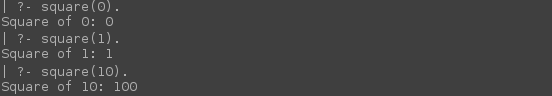
\includegraphics[width=150mm]{img/square}
  \caption{Результат работы программы}
  \label{fig:square}
\end{figure}


Рассмотрим последовательность рекурсивных вызовов функций на примере \texttt{square(3)}:

\begin{enumerate}
\item \texttt{square(3)}:
  переход к предикату \texttt{square(3, Ret)} (строка 12). 
\item \texttt{square(3, Ret)}: 
  рекурсивный переход к предикату \texttt{square(3-1, Ret)} (строка 8).
\item \texttt{square(3-1, Ret)}: 
  рекурсивный переход к предикату \texttt{square(3-1-1, Ret)}.
\item \texttt{square(3-1-1, Ret)}:
  рекурсивный переход к предикату \texttt{square(3-1-1-1, Ret)}.
\item \texttt{square(3-1-1-1, Ret)}:
  так как \( 3 - 1 - 1 - 1 = 0 \), 
  то выбирается предикат \texttt{square(0, Ret)}, a не \texttt{square(N, Ret)}.
\item \texttt{square(0, Ret)}:
  возвращаемое значение устанавливается равным нулю,
  возврат в родительский предикат (строка 4).
\item \texttt{square(3-1-1, Ret)}:
  возвращаемое значение устанавливается равным \( 0 + 2*(3-1-1) - 1 = 1 \),
  возврат в родительский предикат (строка 9).
\item \texttt{square(3-1, Ret)}:
  возвращаемое значение устанавливается равным \( 1 + 2*(3-1) - 1 = 4 \),
  возврат в родительский предикат.
\item \texttt{square(3, Ret)}: 
  возвращаемое значение устанавливается равным \( 4 + 2*(3) - 1 = 9 \),
  возврат в родительский предикат.
\item \texttt{square(3)}: 
  печать значения \texttt{Ret} (строка 13).
\end{enumerate}

Отметим, что данный подход неприменим для вычисления квадратов
больших значений аргументов, поскольку число рекурсивных вызовов 
предиката \texttt{square} линейно зависит от значения аргумента,
а размер системного стека является величиной постоянной.

\pagebreak
\subsection{Программа вычисления суммы  \( \sum_{i=1}^N i \)}

Задание: разработать программу для рекурсивного определения суммы
\( 1 + 2 + 3 + 4 + \dots + N \) для произвольного 
целого положительного \( N \).

Исходный код разработанной программы представлен на
рисунке~\ref{lst:sum}.

\lstinputlisting[style=source_code,
                 caption=Исходный код программы,
                 language=prolog,label=lst:sum]{code/sum.pro}

Пример работы программы представлен на рисунке~\ref{fig:sum}.

\begin{figure}[h!]
  \centering
  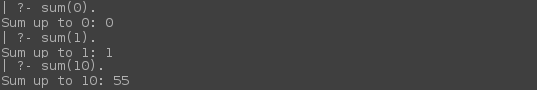
\includegraphics[width=150mm]{img/sum}
  \caption{Результат работы программы}
  \label{fig:sum}
\end{figure}


\pagebreak
\subsection{Программа вычисления \( \min(A, B, C) \)}

Текст задания: разработать программу для рекурсивного определения 
\( \min(A, B, C) \).

Исходный код разработанной программы представлен на
рисунке~\ref{lst:min}.

\lstinputlisting[style=source_code,numbers=left,numberstyle=\texttt,xleftmargin=2.5em,
                 caption=Исходный код программы,
                 language=prolog,label=lst:min]{code/min.pro}

Пример работы программы представлен на рисунке~\ref{fig:min}.

\begin{figure}[h!]
  \centering
  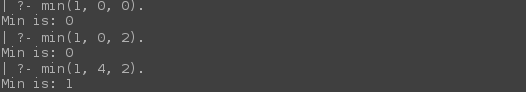
\includegraphics[width=150mm]{img/min}
  \caption{Результат работы программы}
  \label{fig:min}
\end{figure}


\pagebreak
\subsection{Программа организации конечного цикла}

Задание: изменить программу~\ref{lst:repeat} так,
чтобы число вводов пароля было не более 3.

Исходный код разработанной программы представлен на
рисунке~\ref{lst:prompt}.

\lstinputlisting[style=source_code,numbers=left,numberstyle=\texttt,xleftmargin=2em,
                 caption=Исходный код программы,
                 language=prolog,label=lst:prompt]{code/prompt.pro}

Пример работы программы представлен на рисунке~\ref{fig:prompt}.

\begin{figure}[h!]
  \centering
  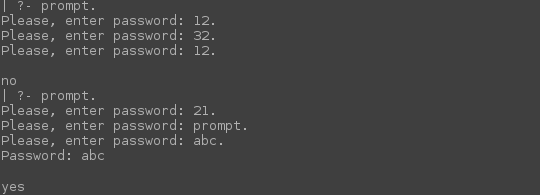
\includegraphics[width=150mm]{img/prompt}
  \caption{Результат работы программы}
  \label{fig:prompt}
\end{figure}


%%% Первый неверный ввод

Рассмотрим работу интерпретатора Prolog, обрабатывающего предикат \texttt{prompt} 
в случае первой попытки ввода неверного значения:

\begin{enumerate}
\item \texttt{prompt}:
  переход к предикату \texttt{loop(3)} (строка 4). 
\item \texttt{loop(3)}:
  проверка \( 3 > 0 \), возврат \texttt{true} в родительский предикат (строка 11). 
\item \texttt{prompt}:
  вывод предложения ввести значение, чтение прочитанного значения,
  сравнение его с предикатом \texttt{abc}. 
  Так как пользователь ввел неверное значение, последнее выражение возвращает
  \texttt{false}, поэтому Prolog переходит ко второму определению
  предиката \texttt{loop} (строки 5--7).
\item \texttt{loop(3)}:
  проверка \( 3 > 0 \),
  рекурсивный переход к предикату \texttt{loop(3-1)},
  определенному выше (строка 15).
\end{enumerate}

Таким образом, можно утверждать, что каждая неудачная попытка ввода пароля уменьшает
аргумент предиката loop на единицу.

%%% Останов

Рассмотрим работу интерпретатора Prolog, обрабатывающего предикат \texttt{prompt} 
в случае последней попытки ввода неверного значения:

\begin{enumerate}
\item \texttt{prompt}:
  переход к предикату \texttt{loop(0)} (строка 4).
\item \texttt{loop(0)}:
  проверка \( 0 > 0 \), возврат \texttt{false} в родительский предикат (строка 11). 
\item \texttt{prompt}:
  Так как предикат \texttt{loop(0)} возвратил ложное значение, производится попытка
  вычисления значения альтернативной реализации предиката (строка 4). 
\item \texttt{loop(0)}:
  проверка \( 0 > 0 \), возврат \texttt{false} в родительский предикат (строка 14). 
\item \texttt{prompt}:
  Так как предикат \texttt{loop(0)} возвратил ложное значение, при этом больше не осталось
  альтернативных определений предиката \texttt{loop}, значение предиката \texttt{prompt}
  устанавливается равным false, тем самым производится выход из цикла. 
\end{enumerate}

Таким образом, можно утверждать, обработка предиката \texttt{loop(0)} всегда
возвращает ложное значение, тем самым завершая обработку родительского предиката.

%%% Верный ввод

Рассмотрим работу интерпретатора Prolog, обрабатывающего предикат \texttt{prompt} 
в случае первой попытки ввода верного значения:

\begin{enumerate}
\item \texttt{prompt}:
  переход к предикату \texttt{loop(3)} (строка 4). 
\item \texttt{loop(3)}:
  проверка \( 3 > 0 \), возврат \texttt{true} в родительский предикат (строка 11). 
\item \texttt{prompt}:
  вывод предложения ввести значение, чтение прочитанного значения,
  сравнение его с предикатом \texttt{abc}. 
  Так как пользователь ввел верное значение, последнее выражение возвращает
  \texttt{true}, поэтому Prolog переходит к обработке следующего выражения,
  которое представляет собой вывод введенного значения на экран (строки 5--8).
\end{enumerate}

Таким образом, можно утверждать, что каждая удачная попытка ввода пароля 
приводит к выводу его на экран и установлению истинного значения предиката \texttt{prompt}.


\subsection{Программа организации консольного меню}

Задание: с помощью предиката repeat построить простое меню с
двумя пунктами. По одному из них производится завершение программы. 
По другому --- выводится сообщение <<Выбран пункт 1>>.

Исходный код разработанной программы представлен на
рисунке~\ref{lst:menu}.

Пример работы программы представлен на рисунке~\ref{fig:menu}.

\begin{figure}[h!]
  \centering
  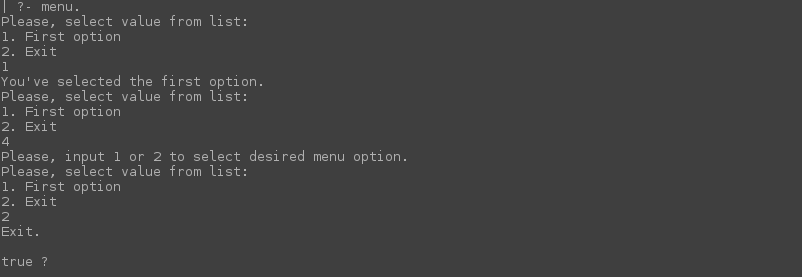
\includegraphics[width=150mm]{img/menu}
  \caption{Результат работы программы}
  \label{fig:menu}
\end{figure}

\pagebreak

\lstinputlisting[style=source_code,
                 caption=Исходный код программы,
                 language=prolog,label=lst:menu]{code/menu.pro}
